\documentclass[paper=a4, fontsize=11pt, UTF8]{article} % A4 paper and 11pt font size
\usepackage[a4paper,left=3.18cm,right=3.18cm,top=2.5cm,bottom=2.5cm]{geometry}
\usepackage{ctex}
%\usepackage[T1]{fontenc} % Use 8-bit encoding that has 256 glyphs
%\usepackage{fourier} % Use the Adobe Utopia font for the document - comment this line to return to the LaTeX default
\usepackage[english]{babel} % English language/hyphenation
\usepackage{amsmath,amsfonts,amsthm} % Math packages
\usepackage{graphicx}
\usepackage{listings}
\usepackage{xcolor}
\usepackage{siunitx}
\usepackage{booktabs}
\usepackage{multirow}
\usepackage{longtable}
\usepackage{hyperref}
\usepackage{graphicx}
\usepackage{float}
\usepackage{amsmath}
\usepackage{listings}
\usepackage{xcolor}
\usepackage{diagbox}

\hypersetup{
    colorlinks,
    citecolor=black,
    filecolor=black,
    linkcolor=black,
    urlcolor=black
}

\lstset{language=C++,%
    %basicstyle=\color{red},
    keywordstyle=\color{blue},%
    extendedchars=false,
    tabsize=4,
    breaklines,
    morekeywords=[2]{1}, keywordstyle=[2]{\color{black}},
    identifierstyle=\color{black},%
    % stringstyle=\color{mylilas},
    commentstyle=\color{green},%
    frame=single,
    showstringspaces=false,%without this there will be a symbol in the places where there is a space
    numbers=left,%
    numberstyle={\small \color{black}},% size of the numbers
    numbersep=9pt, % this defines how far the numbers are from the text
    emph=[1]{for,end,break},emphstyle=[1]\color{red}, %some words to emphasise
    escapeinside=``
}

% \setlength\parindent{0pt}
\title{\fontsize{18}\baselineskip Ensemble Learning Report}

\author{王 \; 琛 \quad 2016011360 \quad 计65}
\date{\normalsize\today} % Today's date or a custom date

\begin{document}

\maketitle % Print the title

\fontsize{11pt}{18pt}\selectfont
%\newpage

\section{Goal}
Given a set of reviews on Amazon website, each instance in the set contains text for the review, id of the product, number of up votes (votes\_up), number of total votes (votes\_all) etc. And reviews with votes\_up / votes\_all $\ge$ 0.9 are considered as good ones and labeled as 1, otherwise the label is 0. The goal is to establish a hypothesis function that predict the label of a review.

The algorithm is confined to be ensemble learning algorithms, specfically Bagging \& Adaboost M1 with SVM \& Decision Tree.


\section{Experiment Design}
Experiment Design consists of following parts:
\begin{itemize}
    \item Process the raw text
    \item Extract features from data
    \item Train the model and predict
\end{itemize}

\subsection{Data Processing}
The data need to be preprocessed is mainly the content of each review, namely a paragraph of English text, which may contains numbers, symbols etc. We need to remove those inrelevant to our analysis. 

First, I converted all letters to lower case and deleted numbers and punctuations. Then, stop words were filtered (stop words are the common words in a language such as "the", "a", "on" that with little real meaning). Next procedure is stemming -- reduce words to their word stem, base or root form to eliminate the influence of word form.

\subsection{Feature Extraction}
To extract feature from text, the most important part is to use the information of words, i.e. where a certain word appears, the frequency of a word etc. I used bag-of-words (BOW) model, tf-idf model and word2vec in this experiment.

\subsubsection{BOW}
BOW first constructs a vocabulary set from text. Note that some words in test set may not appear in train set, therefore, I constructed the vocabulary combining both test set and train set. With vocabuary set, each text can be represented by a vector or one-dimension matrix. Each item in the vector denontes how many times the corresponding word appears in the whole text. 

In python, BOW can be implemented by CountVectorizer :
\begin{lstlisting}[language=python]
    vectorizer = CountVectorizer(stop_words="english")
    X = vectorizer.fit_transform(corpus)
    X_test = vectorizer.transform(test)
\end{lstlisting}

The following shows the scatter of word count. The vertical axis represents how many times the word appears,  and the horizontal axis represents how many words appears with this count. We can see most words appear for a hundred of times. Words appear for 10000+ times is rare.

\begin{figure}[H]
	\centering
	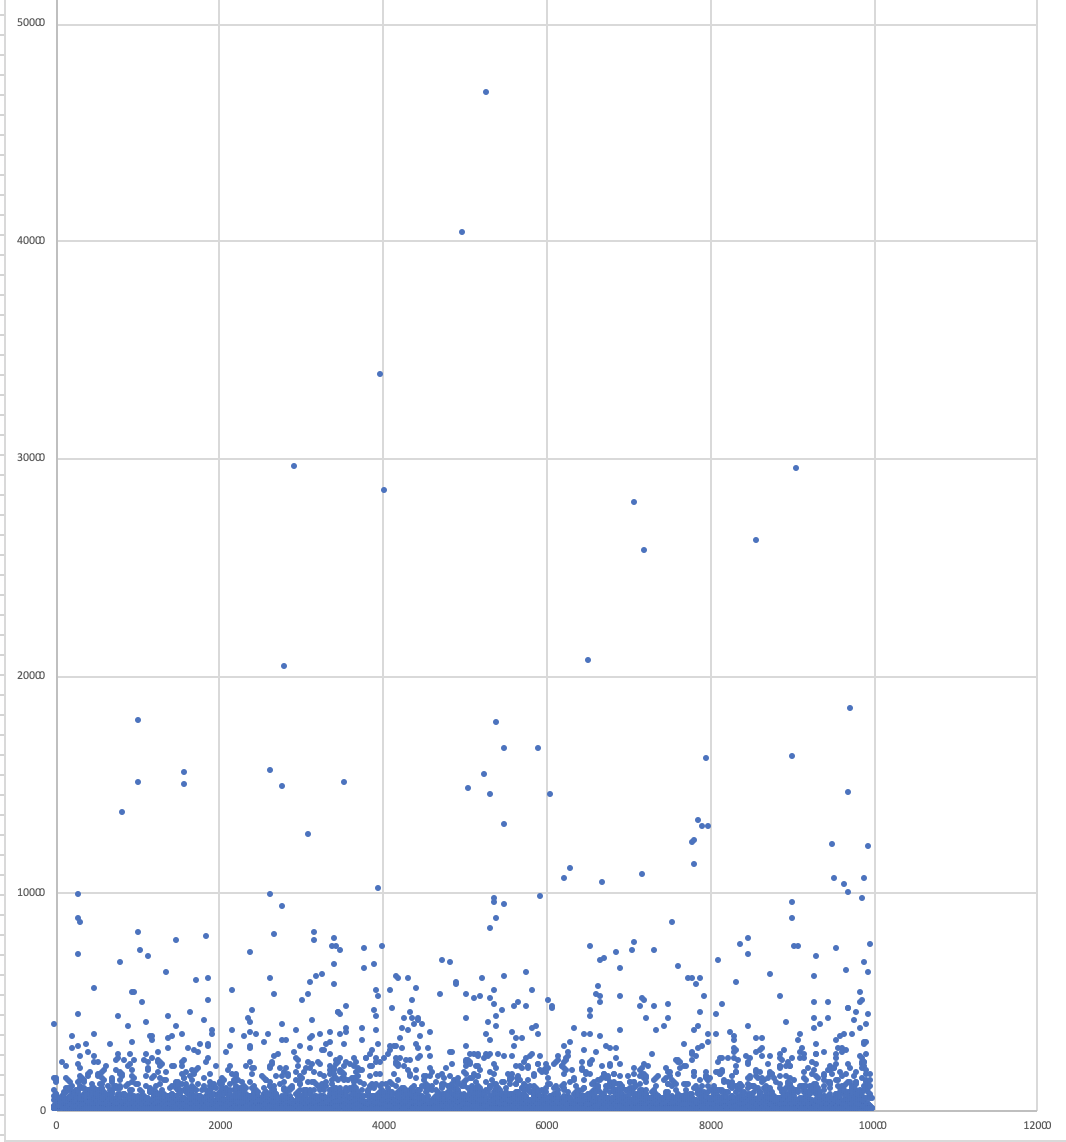
\includegraphics[scale=0.5]{./photos/frequency.png}
	\label{fig1}
\end{figure}

\subsubsection{TF-IDF}
The problem with BOW is that some highly frequency words may not contain as much information as other domain specific words, though we have already filtered stop words. So another approach that rescales the frequency of words by how often they appear in each document (in our case, each review). TF-IDF is Term Frequency - Inverse Document Frequency where TF is the frequency of the word in current document and IDF is how rate the words is across documents. 

Equations for TF-IDF
$$
tf(t, d) = N(t, d) / || D ||
$$
$$
idf(t) = log(N/ df(t))
$$
$$
tfidf(t, d) = tf(t, d)*idf(t)
$$
wherein tf(t, d) = term frequency for a term t in document d, || D || = Total number of term in the document, N(t, d) = number of times a term t occurs in document d.

Similarly in python, we can use `TfidfVectorizer` just like the way how `CountVectorzier` is used.

However, there are still limitations for TF-IDF. In TF-IDF, we ignore the word order thus ignoring the context and words with low IDF may just mean they are important.

\subsubsection{word2vec}
Word2vec is model that is used to produce word embeddings. Different from BOW and TF-IDF, Word2vec derives a vector representation for each word, and the dimension for the vector is fixed. Word2vec contains two types of training method -- CBOW and Skip-gram. Both methods use a three-layered neural network. To get the vector for a paragraph, I just added the vector of every word in the paragraph together and took the average. Word2vec can be found in python gensim module.

\subsection{Train the model}
We are required to implement ensemble learning algorithms in this experiment -- bagging and adaboost. 
\begin{itemize}
    \item Bagging: In Bagging, we get a hypothesis from T existing hypoethesis. The most important concept in Bagging is bootstrap sampling, which draws examples uniformly at random with replacement. We utilize bootstrap sampling on primary train set to get a equal-size new train set.  Then, training is performed on this set. The final predict comes from voting from the T hypothesis. Since we use AUC for scoring, I averaged the probability each classifier predicted.
    \item Adaboost: Adaboost can be divided into Adaboost M1 and Adaboost M2. The core idea of Adaboost M1 is to learn from mistakes. In each iteration, we increase the relative weight of misclassified training examples and decrease the weight of correctly classified ones. Similar to Bagging, we also use hypothesis in each iteration to predict. The difference is that each classifier is assigned a weight when predicting.
\end{itemize}

\section{Experiment result}

I tested single Naive Bayes, SVM, Decision Tree and also combines them with bagging and adaboost and get the following result.

\subsection{Single Classifier}
Use single classifier (Split the train set 9:1, 9 for train and 1 for validation)
\begin{table}[H]
\centering
\begin{tabular}{|@{}c|c|c|c|}
	\hline
	\diagbox[width=8em,trim=l]{Method}{Classifier} & NB & DTree & SVM\\
	\hline
    TF-IDF & 60.34 & 64.09 & 79.2\\
    \hline
    BOW & 72.88 & 66.40 & 71.93\\
    \hline
    Word2vec & & 60.16 & 75.36\\
    \hline
\end{tabular}
\label{table1}
\caption{The result of single classifier}
\end{table}
Note that the result Word2vec contains negative item, so it cannot be used in Naive Bayes. From the above table, it is not hard to find that SVM with TF-IDF outperforms all other situations by at least 4\% increase in accuracy. 

\subsection{Adaboost and Bagging}
Futher, I got the result of the four combinations and changed the number of iterations in both adaboost and bagging and get the following result.
(Split the train set 9:1, 9 for train and 1 for validation, use TF-IDF)
\begin{figure}[H]
	\centering %图片全局居中
	%并排几个图,就要写几个minipage
	\begin{minipage}[b]{0.45\textwidth} %所有minipage宽度之和要小于1,否则会自动变成竖排
		\centering %图片局部居中
		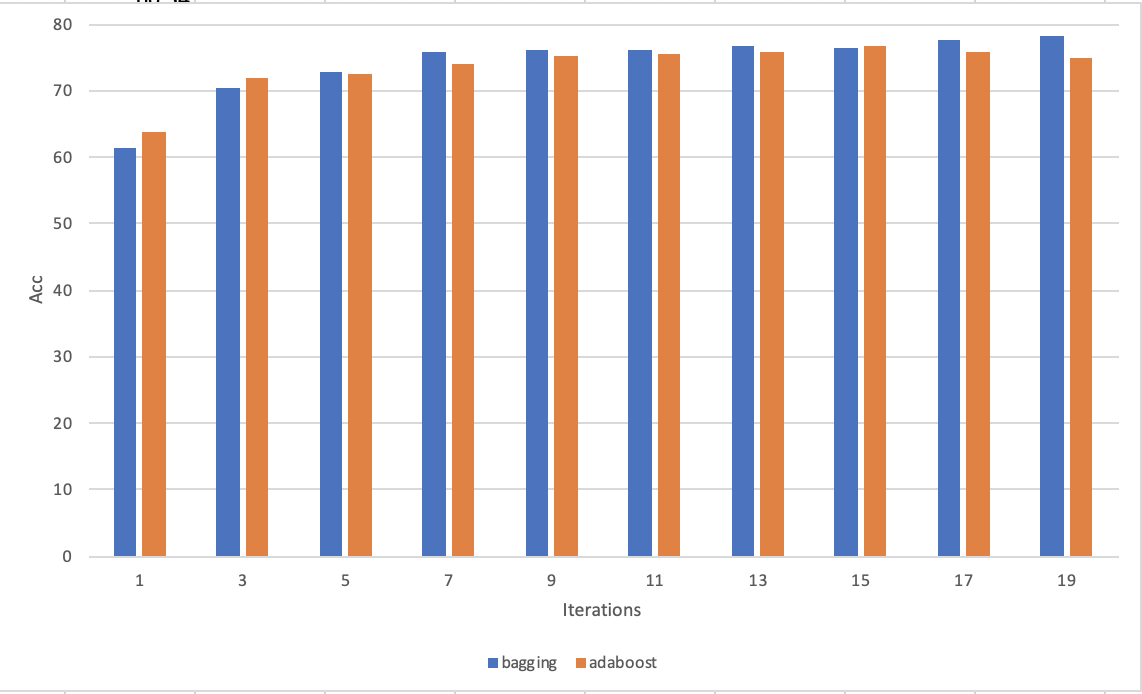
\includegraphics[scale=0.3]{./photos/dtree1.png} %此时的图片宽度比例是相对于这个minipage的,不是全局
	\end{minipage}
	\begin{minipage}[b]{0.45\textwidth} %所有minipage宽度之和要小于1,否则会自动变成竖排
		\centering %图片局部居中
		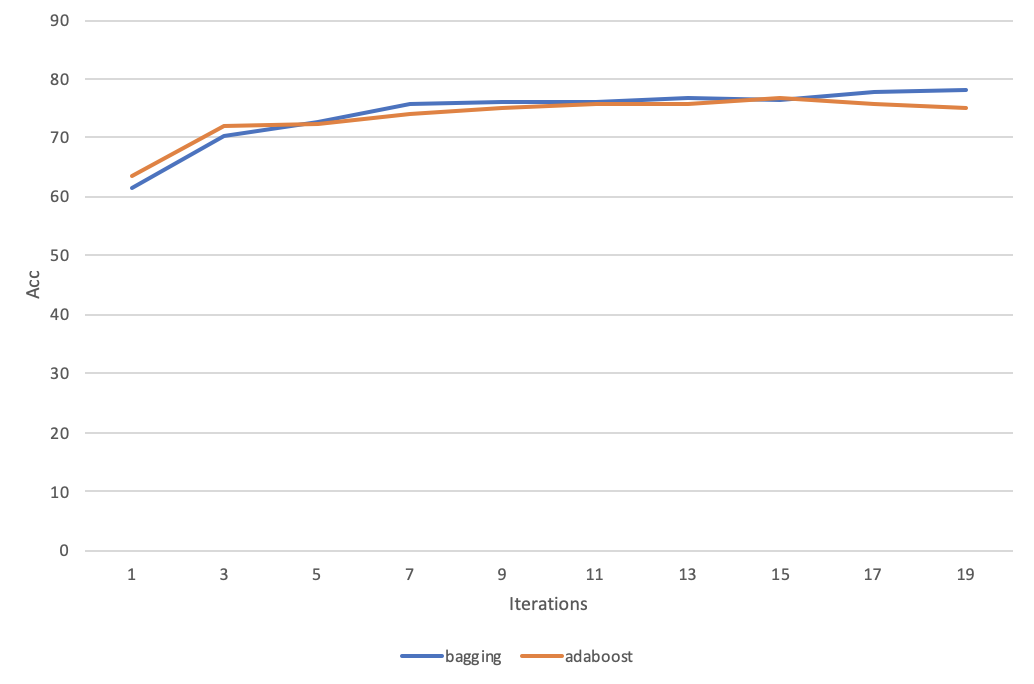
\includegraphics[scale=0.3]{./photos/dtree2.png}%此时的图片宽度比例是相对于这个minipage的,不是全局
    \end{minipage}
    \caption{Bagging and Adaboost for Dtree}
    \label{dtree}
\end{figure}

\begin{figure}[H]
	\centering %图片全局居中
	%并排几个图,就要写几个minipage
	\begin{minipage}[b]{0.45\textwidth} %所有minipage宽度之和要小于1,否则会自动变成竖排
		\centering %图片局部居中
		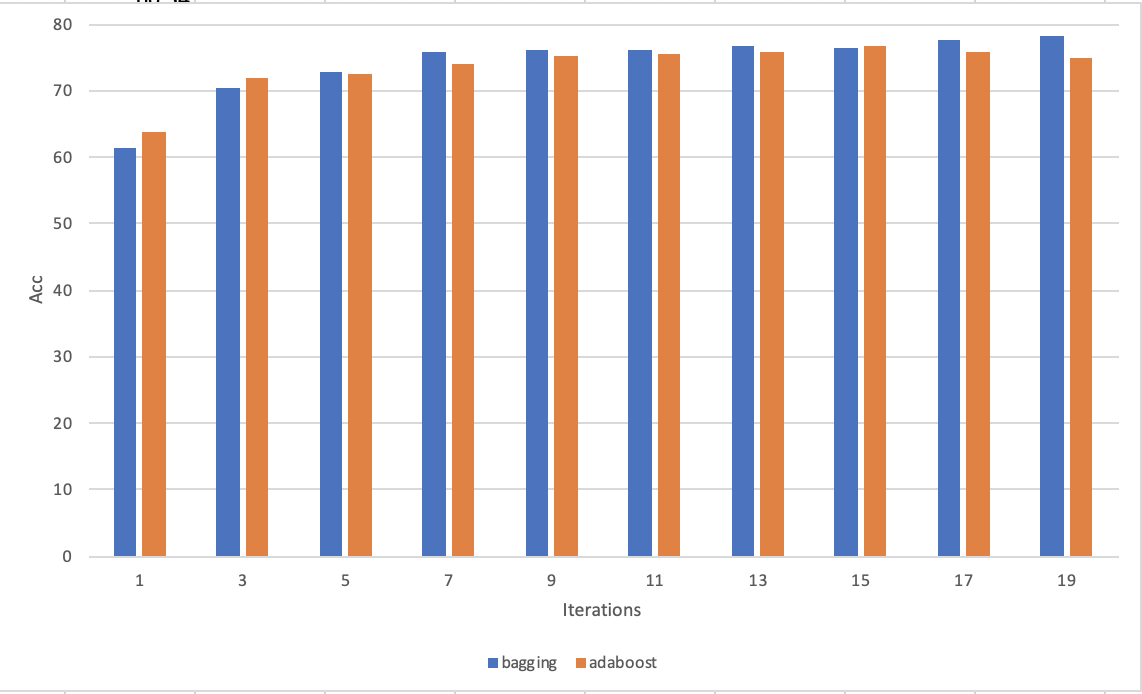
\includegraphics[scale=0.3]{./photos/dtree1.png} %此时的图片宽度比例是相对于这个minipage的,不是全局
	\end{minipage}
	\begin{minipage}[b]{0.45\textwidth} %所有minipage宽度之和要小于1,否则会自动变成竖排
		\centering %图片局部居中
		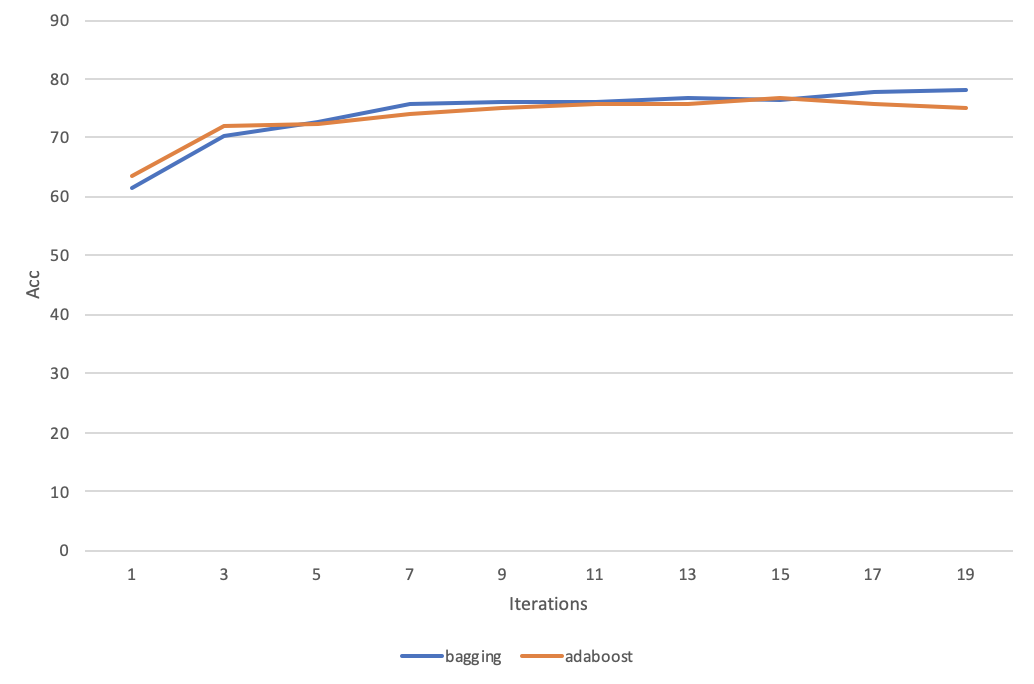
\includegraphics[scale=0.3]{./photos/dtree2.png}%此时的图片宽度比例是相对于这个minipage的,不是全局
    \end{minipage}
    \caption{Bagging and Adaboost for SVM}
    \label{svm}
\end{figure}

\begin{figure}[H]
	\centering
	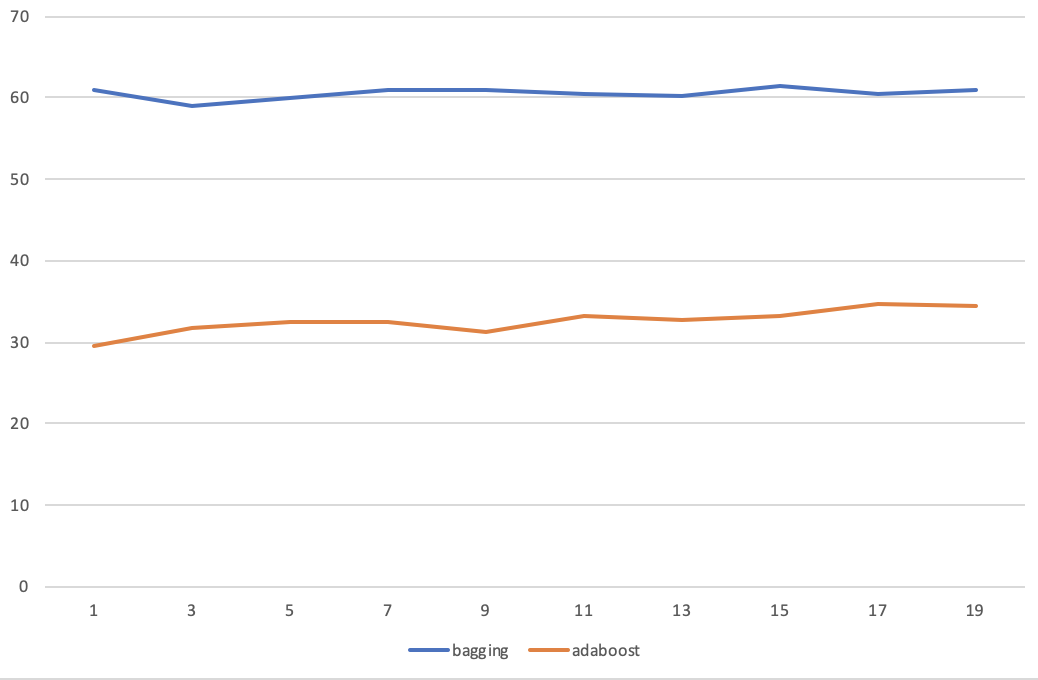
\includegraphics[scale=0.5]{./photos/nb.png}
    \label{nb}
    \caption{Bagging and Adaboost for NB}
\end{figure}
Note that in the above test, Adaboost doesn't abort loop when error rate exceeds 0.5. I just tried to make it to run the full rounds. In fact, adaboost will stop at the fourth round for SVM and maintains accuracy around 79\%, second round for NB. And it will not stop for DTree. 

For precise value, please refer to result.xlsx.

\subsection{Kaggle Score}
Use 100 percent train set, TF-IDF and overall column.

Kaggle id: easymoneysniper, rank: 7
\begin{center}
    \begin{tabular}{c|c|c}
        \hline
        Classifier & Iterations & Score\\
        \hline
        Bagging-SVM & 13 & 80.703\\
        \hline
        Adaboost-SVM & 17 & 80.243\\
        \hline
        Bagging-DTree & 19 & 77.531\\
        \hline
        Adaboost-DTree & 15 & 77.144\\
        \hline
    \end{tabular}
\end{center}
The selection of number of iterations in adaboost and bagging is based on the result of last subsection. 

\section{Discussion}
\subsection{Observations}
We can see from \ref{table1} that each classifier performs differently in different conditions. NB and DTree performs better using BOW, while SVM performs best on TF-IDF. 
\begin{itemize}
    \item When using BOW, Bayes is better than Decision tree and SVM. That is because bayes calculates the probability based on word frequency, that also explains why NB on TF-IDF is the worst. Because TF-IDF has scaled word count.
    \item In general, SVM is the best. Due to its geometric meaning, it is really suitable for binary classification, whereas Decision Tree isn't.
    \item Ensemble Learning has much greater effect on Dtree than on SVM and Bayes. That's because SVM and Bayes is quite steady, but DTree is not stable.
\end{itemize}

The best combination is SVM with bagging because using TF-IDF is more suitable for the short reviews and SVM is just great for binary classification. With bagging, the performance is further improved. The difference between bagging and adaboost for SVM is ignorable.

\subsection{Comparison of Bagging and Adaboost}
We know that the core of bagging is to do bootstrap sampling and adaboost is to use weight. In our case, Bagging is better than Adaboost. This contradicts to my previous consideration. I think that Adaboost can learn from mistakes, so it is better especially for unstable algorithms like Dtree, but the result is just the other way round. I guess it may because in Adaboost, every classifier has differnt weight. But in my implementation, the classifier is the same, so weight doesn't matter. Therefore, the strength of Adaboost is not revealed.

\subsection{The influence of iterations}
From figures in Section 3.2, the more iterations for bagging, the better the result will be on validation set, particularly for Decision Tree, although some fluctuations may occur. Of course, for SVM and NB, the influence of iteration is quite little, since both algorithms is stable enough.

\subsection{Effect of different features}
Test conditions: Bagging, SVM, TF-IDF, Train : Validation = 9 : 1
\begin{center}
    \begin{tabular}{l|c|c}
        \hline
        Classifier & Iterations & Score\\
        \hline
        Neither & 13 & 76.68\\
        \hline
        Review ID & 13 & 78.37\\
        \hline
        Overall & 13 & 80.88\\
        \hline
        asin & 13 & 78.44 \\
        \hline
        Overall and asin & 13 & 80.08 \\
        \hline
        Overall, Review ID and asin & 13 & 80.00\\
        \hline
    \end{tabular}
\end{center}
From the table, we can see that adding only overall is the best. Adding only one feature will definitely be better, but adding them together is not. Maybe it is because that too many features influence each other.

\section{Summary}
In the experiment, I implemented ensemble learning algorithms, namely Bagging and Adaboost.M1. I spent a lot of time and made many attempts, trying different combinations of different classifier and extraction techniques. I am aware that some results may not correspond to your speculations at all. For example, you may not improve your results even if you include more features that you think are useful. And without preprocessing before BOW and TF-IDF, the result is unexpectedly better, so the form of words also contains information. At first, I converted the sparse matrix got from TfidfVectorizer to two-dimensional array and passed it to classifier, the training process is really long and boring. With full training size, it is even killed by the Operating System. Later, I passed the sparse matrix (CSR form) directly, it consumed less memory and become much faster.


\end{document}
